\documentclass[dvipsnames]{beamer}
\beamertemplatenavigationsymbolsempty
\usetheme{Boadilla}
\usefonttheme[onlymath]{serif}

\usepackage{amsmath}
\usepackage{bm}
\usepackage{bbm}
\usepackage{mathrsfs}
\usepackage{mathtools}
\usepackage[cal=boondoxo]{mathalpha}

% Change horizontal spacing
\setlength{\tabcolsep}{3pt}

\usepackage[none]{hyphenat} % no hyphenation

\usepackage{array}

\usepackage{cancel}

\usepackage[style=authoryear,maxcitenames=2,backend=biber,citetracker=true]{biblatex}
\addbibresource{references.bib}

\usepackage{verbatim}

\usepackage{bigints}

\newcommand{\credit}[2]{\par\hfill \footnotesize #1 credit:~\itshape\citeauthor{#2} (\citeyear{#2})}
\renewcommand{\cite}[1]{(\citeauthor{#1}, \citeyear{#1})}
\newcommand{\citefoot}[1]{\citeauthor{#1} (\citeyear{#1})}
\newcommand{\matr}[1]{#1}

\newcommand{\red}[1]{{\color{red} #1}}

\title[ProLLaMA]
{ProLLaMA: A Protein Large Language Model for Multi-Task Protein Language Processing}
%\subtitle{}
\author[Liuzhenghao Lv et al.]{Lv, Liuzhenghao, Zongying Lin, Hao Li, Yuyang Liu, Jiaxi Cui, Calvin Yu-Chian Chen, Li Yuan, and Yonghong Tian
\\\vspace{2em}Presenter: Gianmarco Midena}
%\institute{Aalto University}
\date[3 July 2024]{Submitted on 26 February 2024 
\\\vspace{2em}3 July 2024}

\begin{document}
\begin{frame}
\titlepage
\end{frame}

\begin{frame}{Multi-task LLMs for Natural vs. Protein Language}
	\begin{center}
		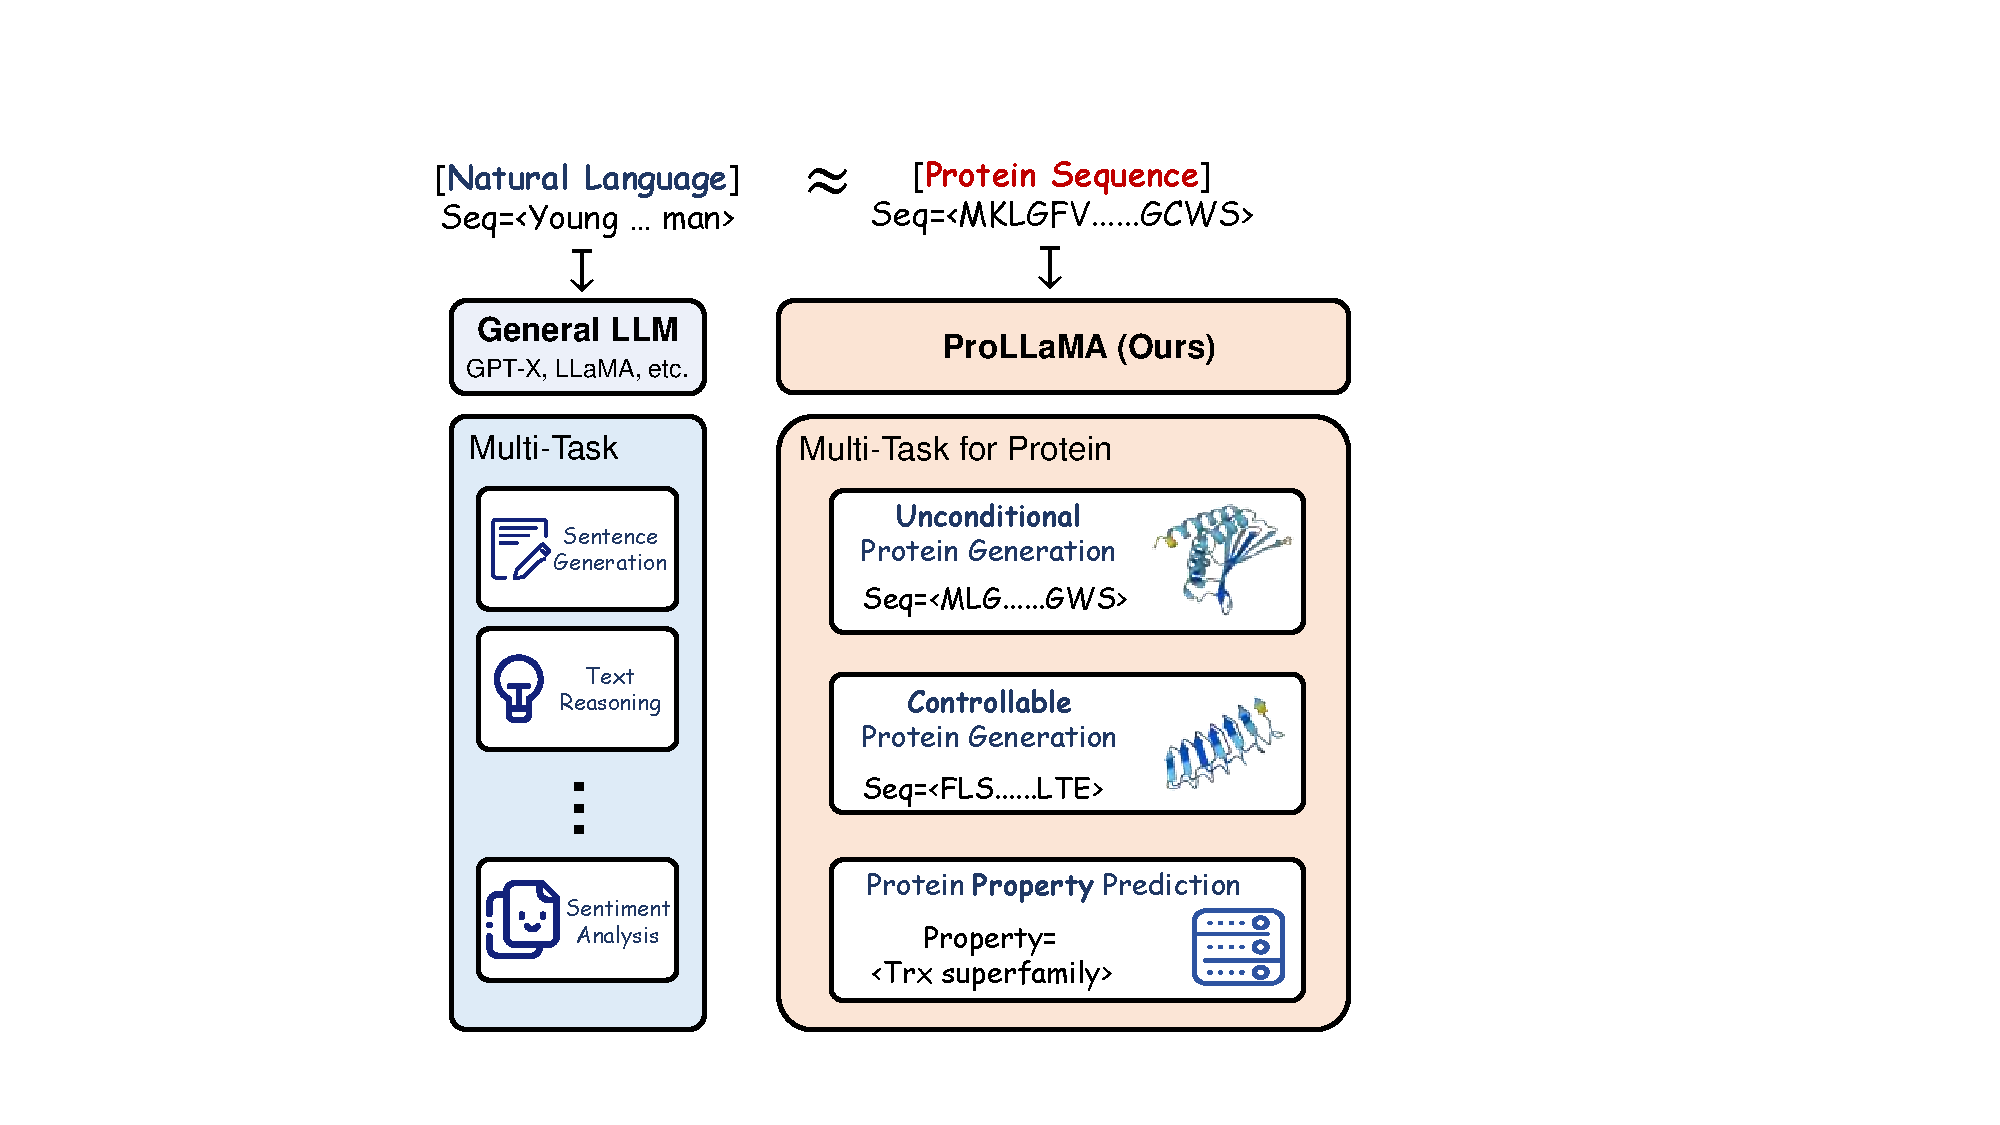
\includegraphics[scale=0.5]{images/multitask_LLMs_NLP_vs_PLP.pdf}
	\end{center}
\end{frame}

\begin{frame}{Model}
	\begin{center}
		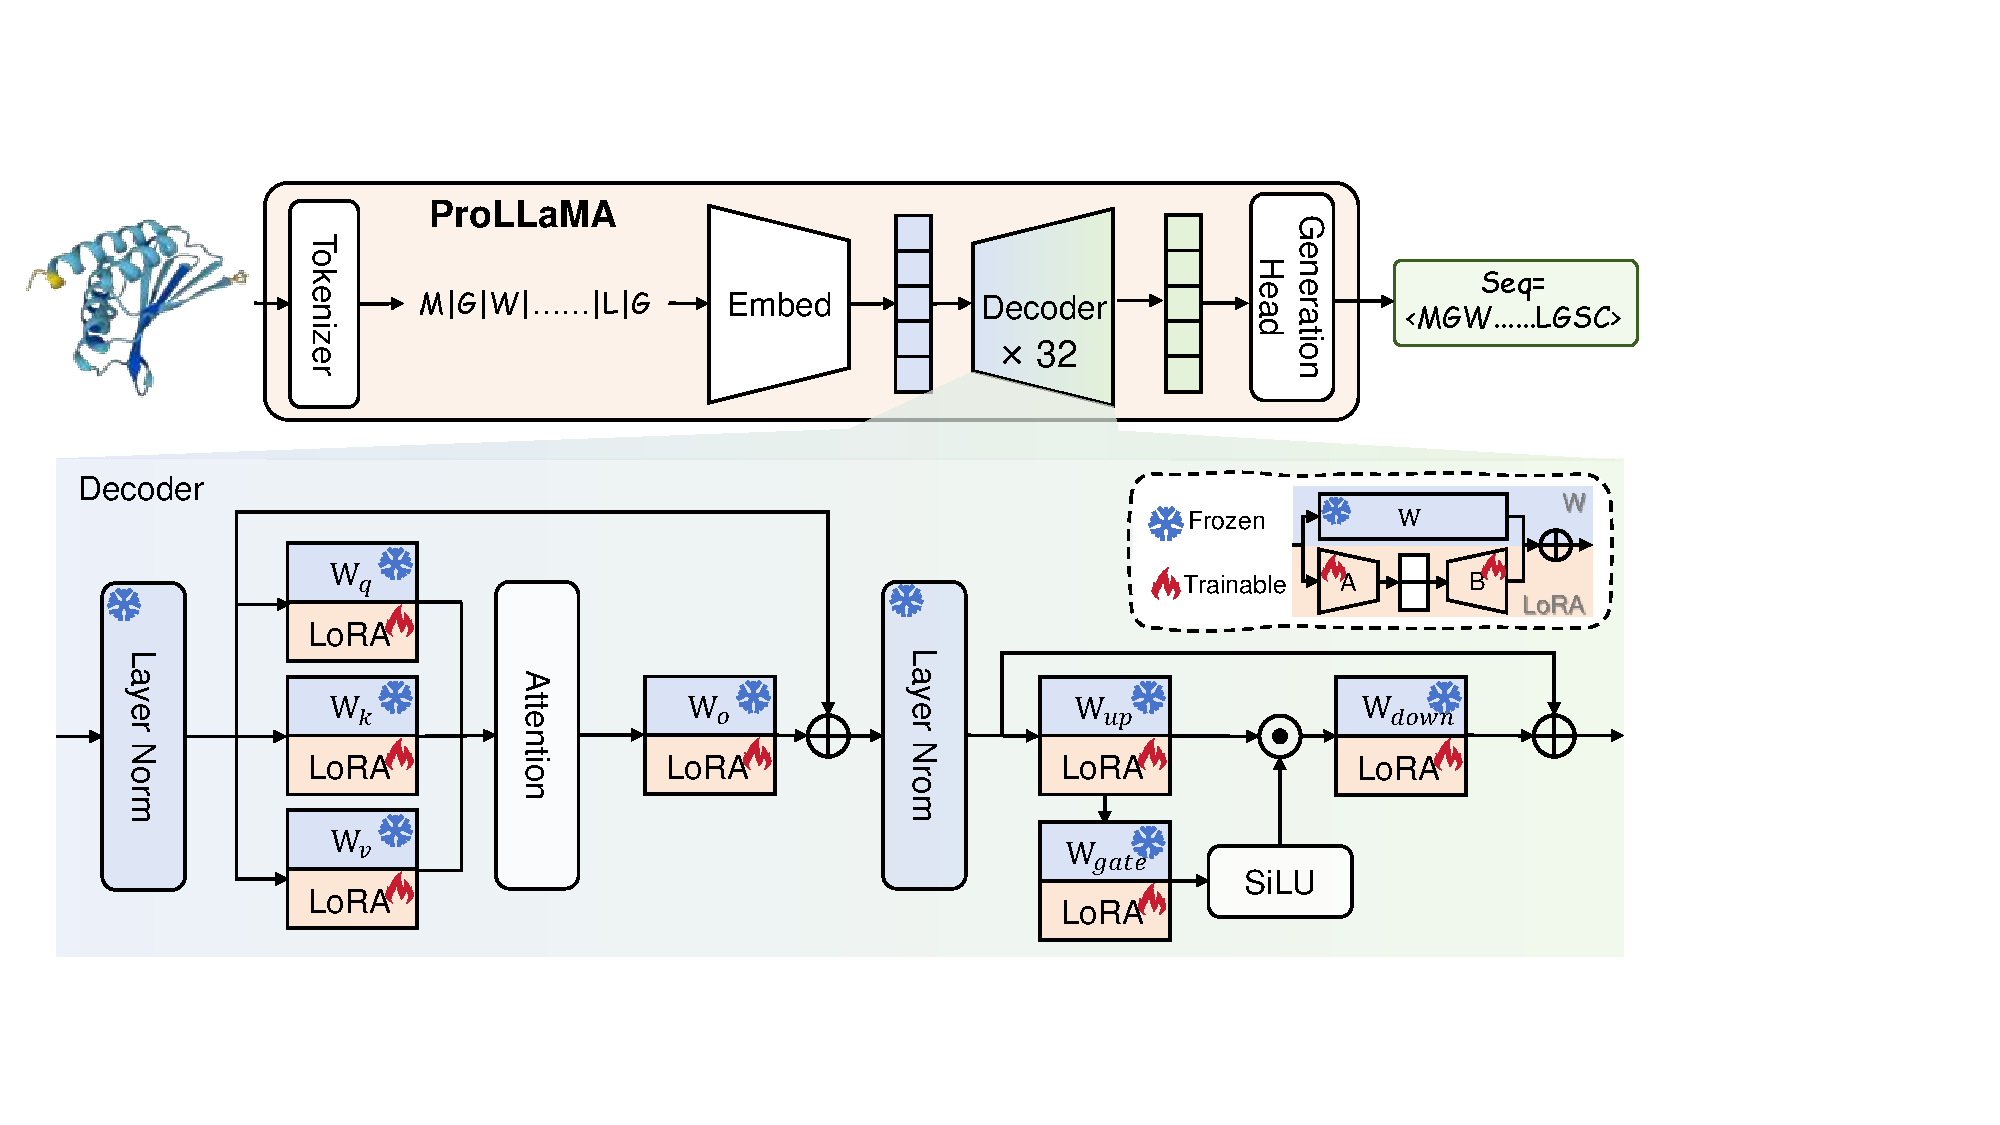
\includegraphics[scale=0.44]{images/model.pdf}
	\end{center}
\end{frame}

\begin{frame}{Training}
	\begin{center}
		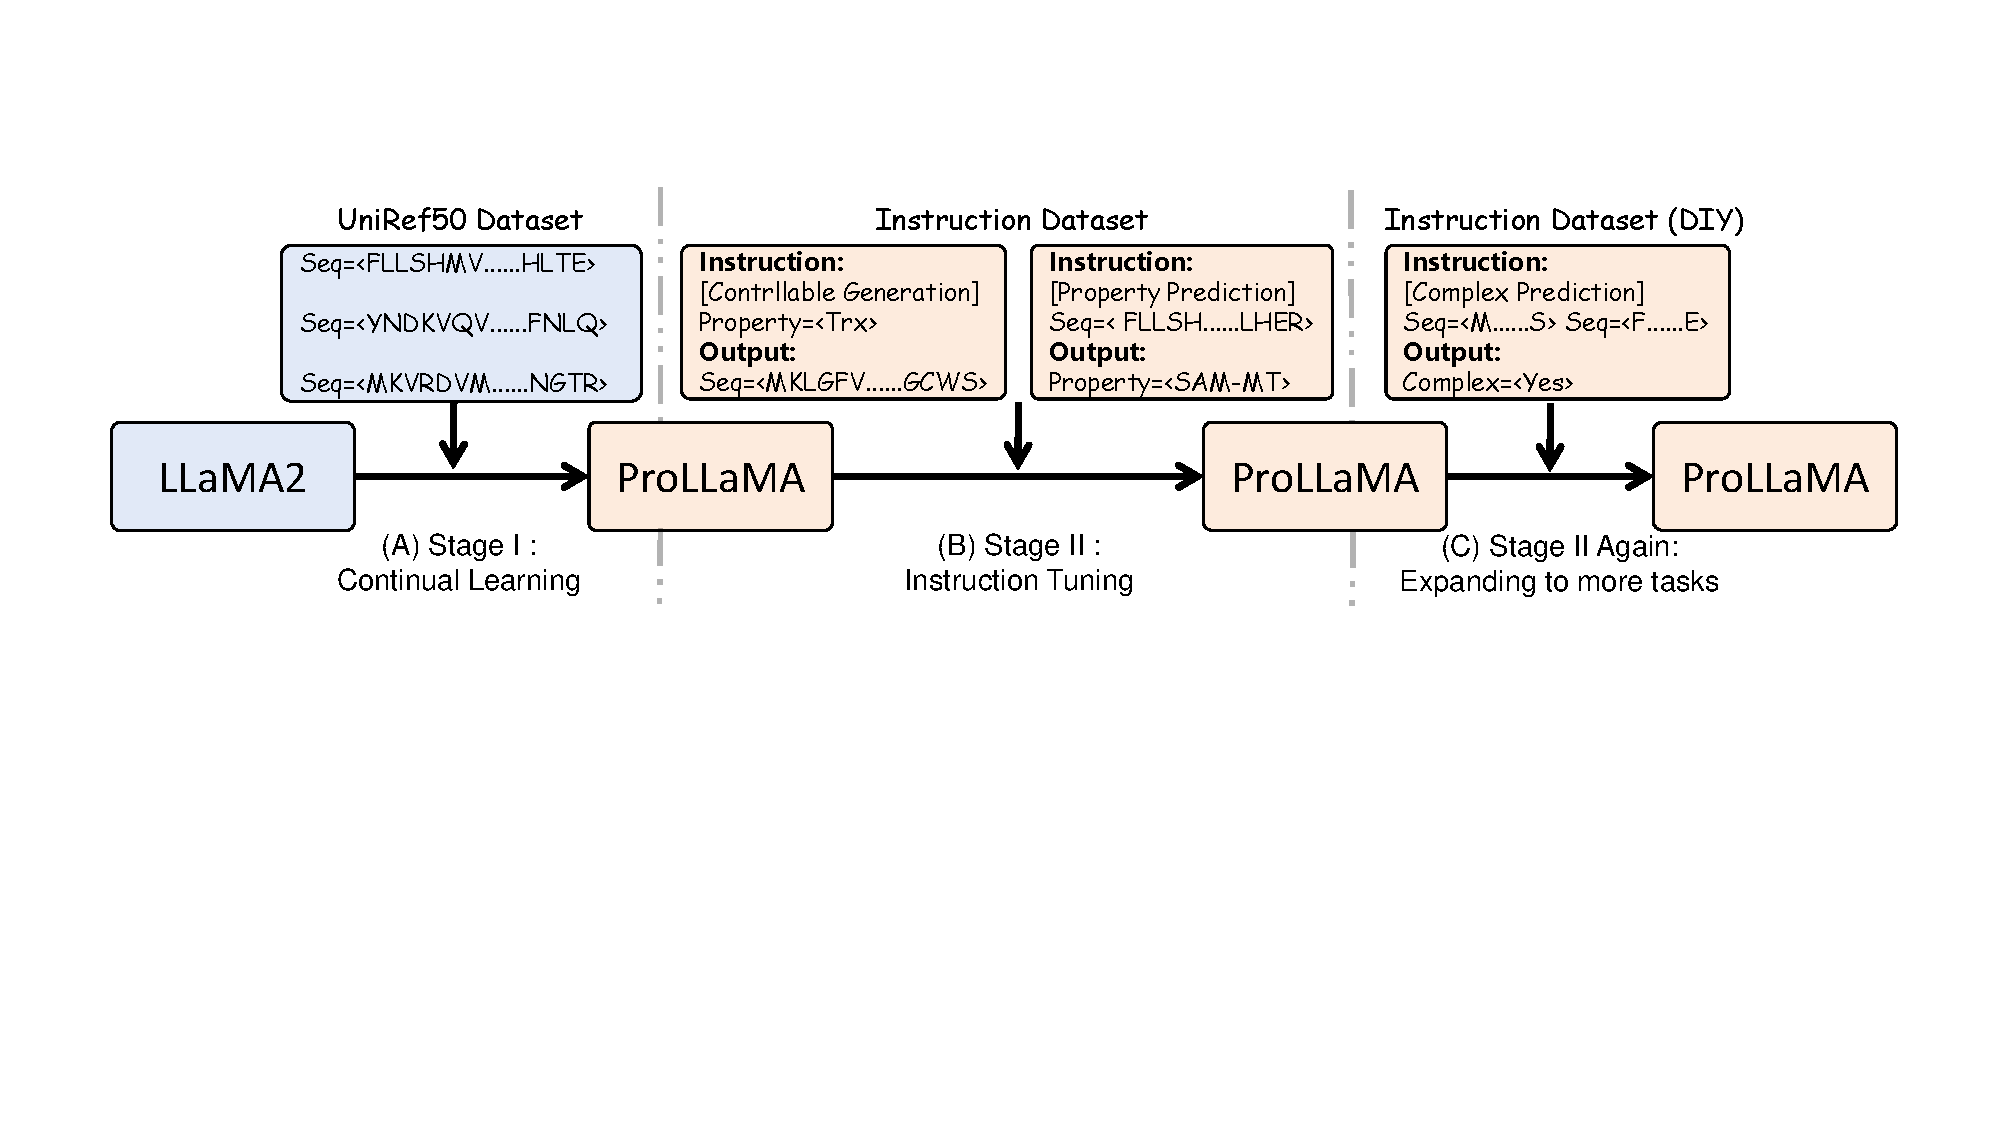
\includegraphics[scale=0.39]{images/training.pdf}
	\end{center}
\end{frame}

\begin{frame}{Proteins Generated by Model}
	\begin{center}
		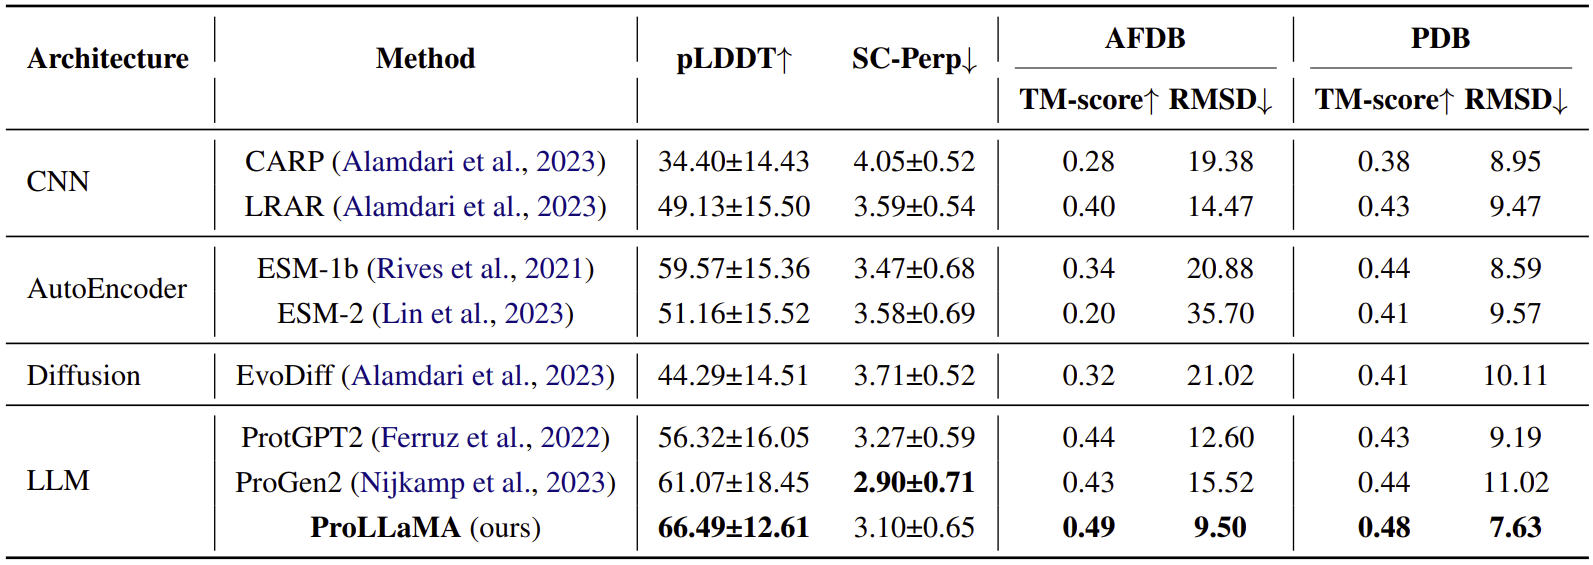
\includegraphics[scale=0.21]{tables/methods_comparison.png}
	\end{center}
\end{frame}

\begin{frame}{Controllable Generation on Four Different Instructions}
	\begin{center}
		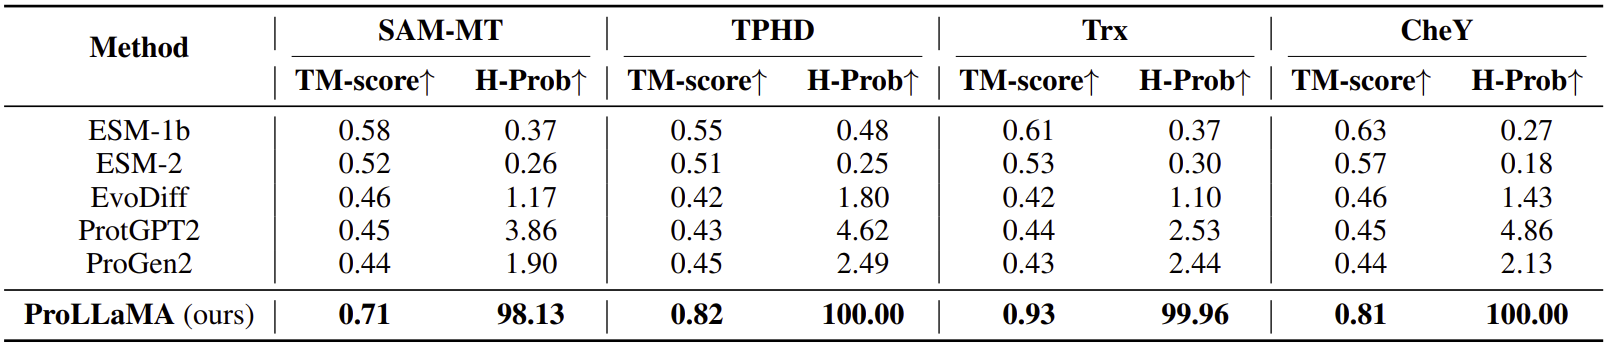
\includegraphics[scale=0.21]{tables/controlled_generation_comparison.png}
	\end{center}
\end{frame}

\begin{frame}{ProLLaMA vs. ESM2 Model (Baseline)}
	\begin{center}
		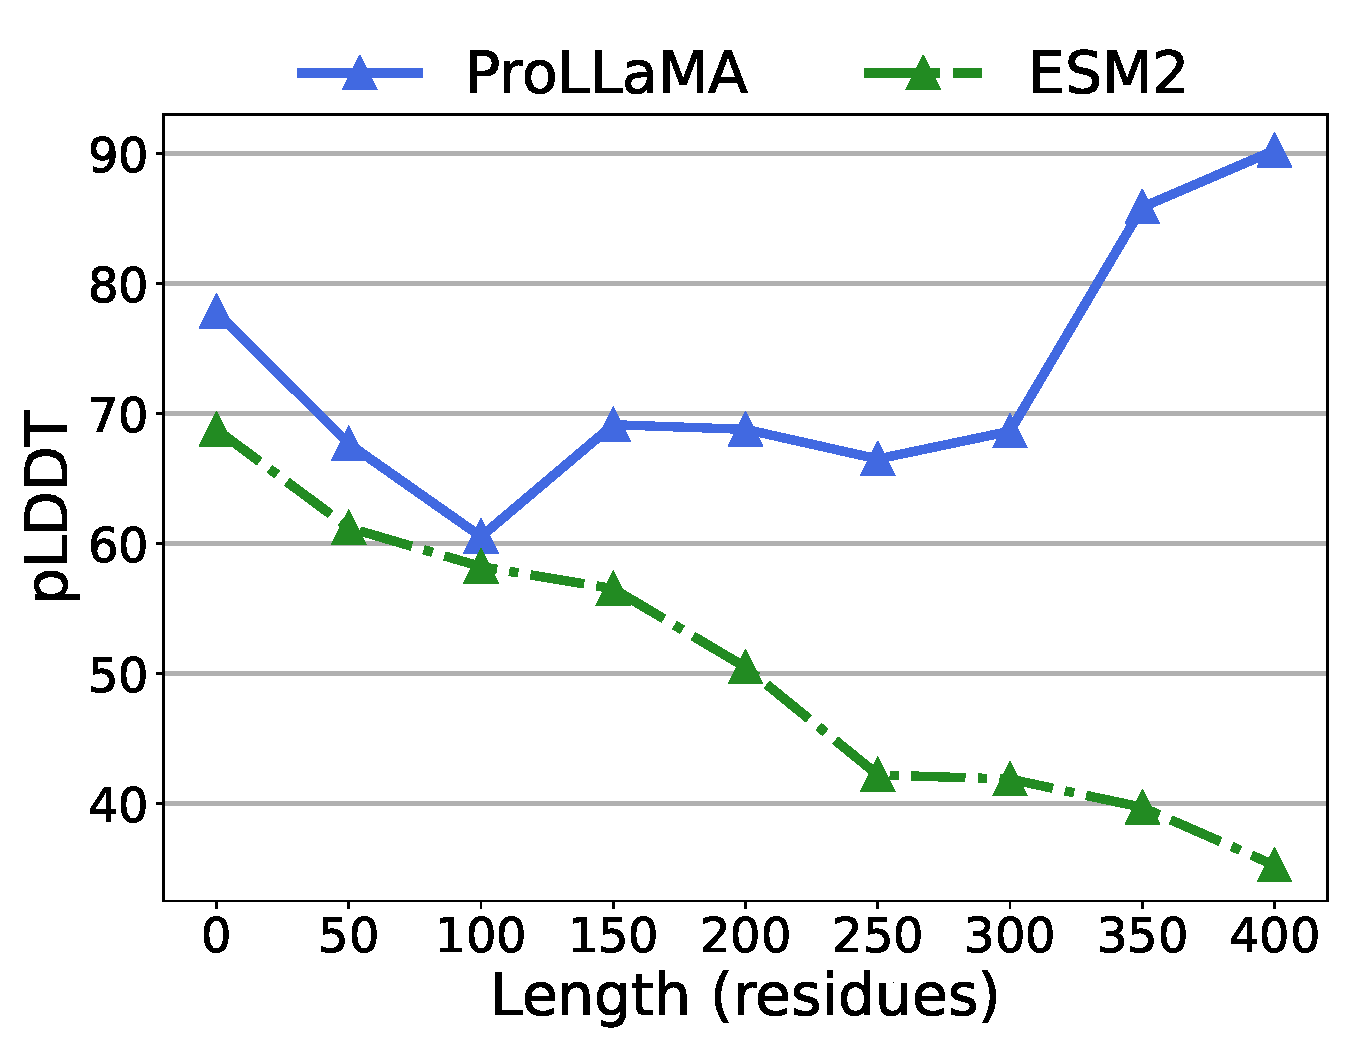
\includegraphics[scale=0.23]{images/combined_length_plddt_zhexiantu.pdf}
		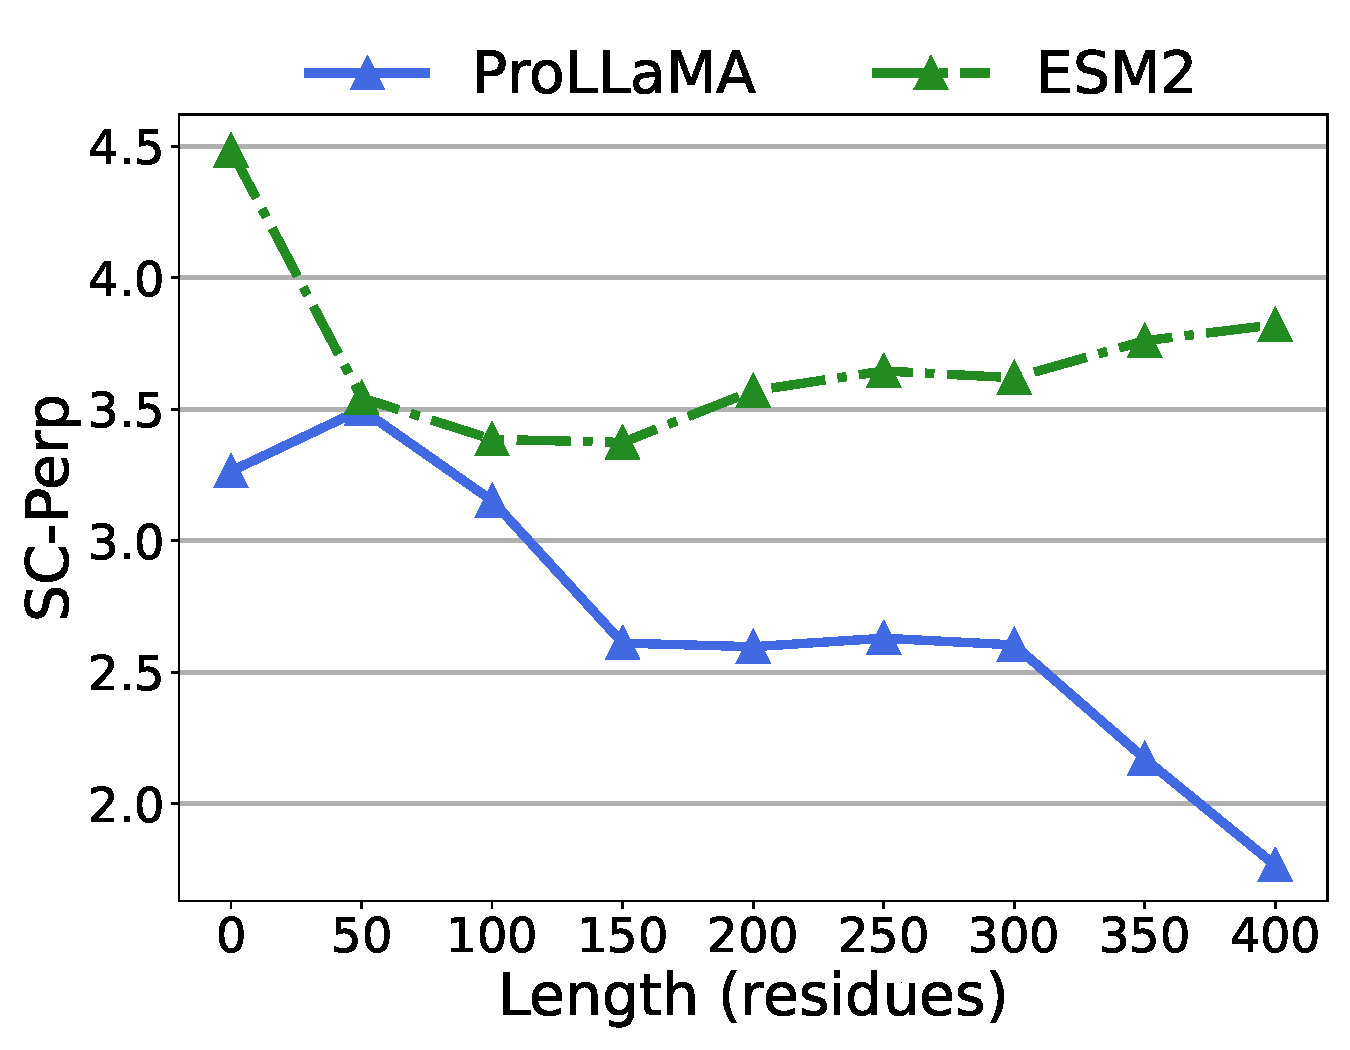
\includegraphics[scale=0.23]{images/combined_length_scperp_zhexiantu.pdf}
		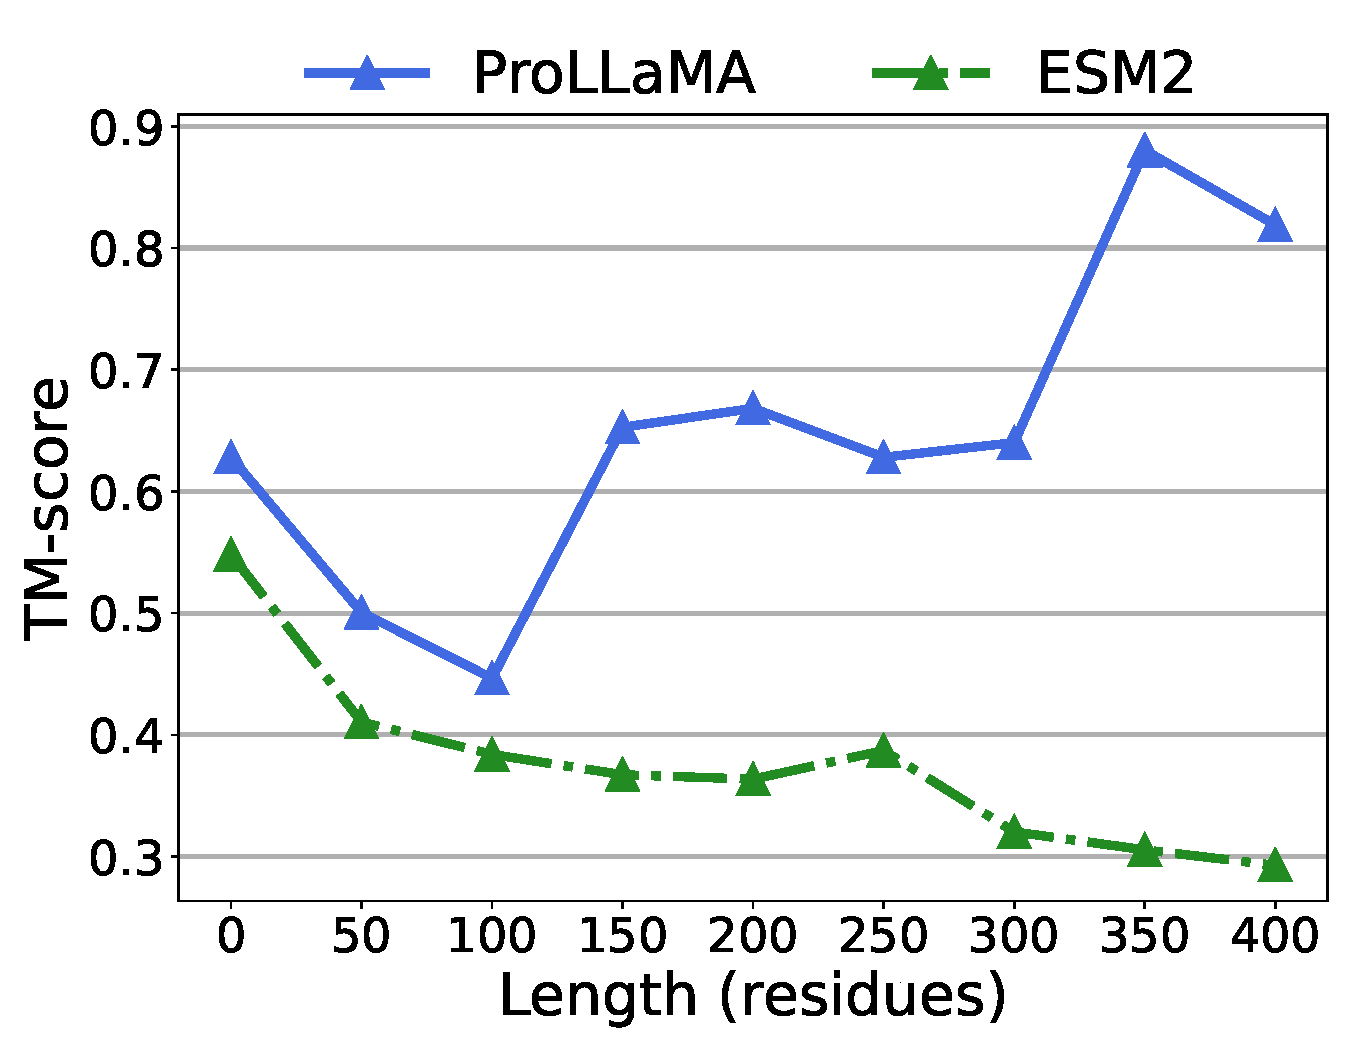
\includegraphics[scale=0.23]{images/combined_length_alntmscore_zhexiantu.pdf}
	\end{center}
\end{frame}

\begin{frame}{Generated vs. Natural Protein}
	\begin{center}
		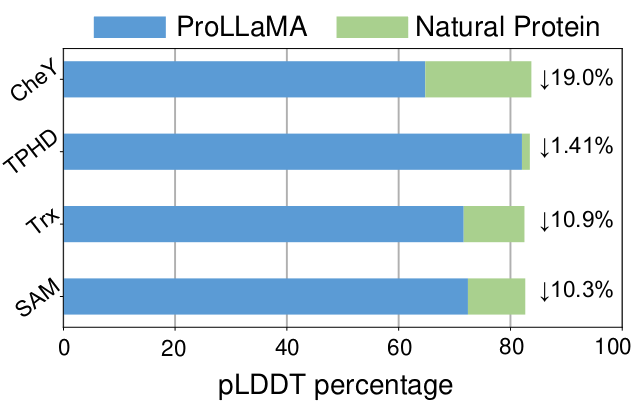
\includegraphics[scale=0.7]{images/d.png}
		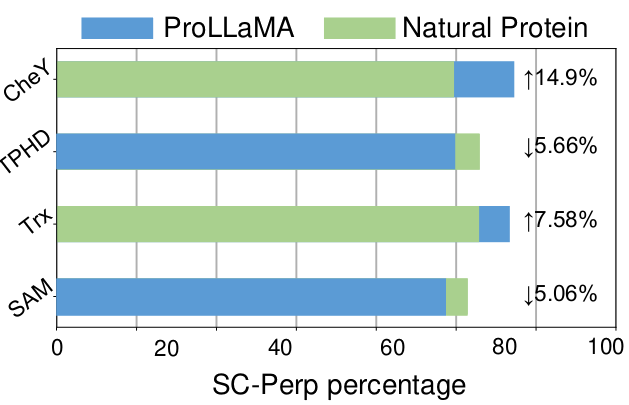
\includegraphics[scale=0.7]{images/e.png}
		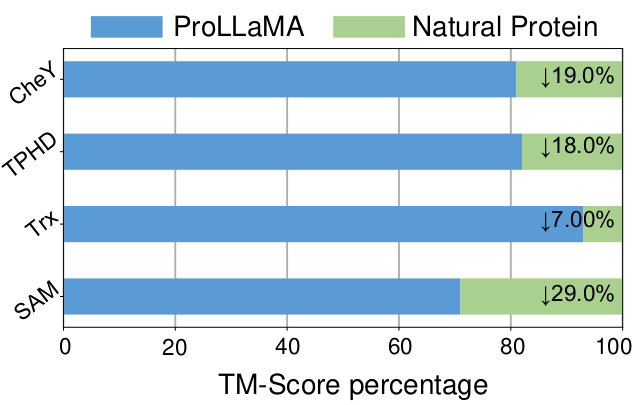
\includegraphics[scale=0.7]{images/f.png}
	\end{center}
\end{frame}

\begin{frame}{Performance in Protein Property Prediction}
	\begin{center}
		\begin{tabular}{cc}\hline
			Property & Accuracy (\%) \\\hline
			OBFD     & 100 \\
			UPF0145  & 100 \\
			NACD     & 100 \\
			U3S      & 100 \\
			CCHC     & 95.24  \\
			Kazal    & 100 \\
			SAM-MT   & 93.67  \\
			TPHD     & 90.84  \\
			Trx      & 94.17  \\
			CheY     & 100 \\\hline
		\end{tabular}
	\end{center}
\end{frame}

\begin{frame}{Protein Visualization}
	\begin{center}
		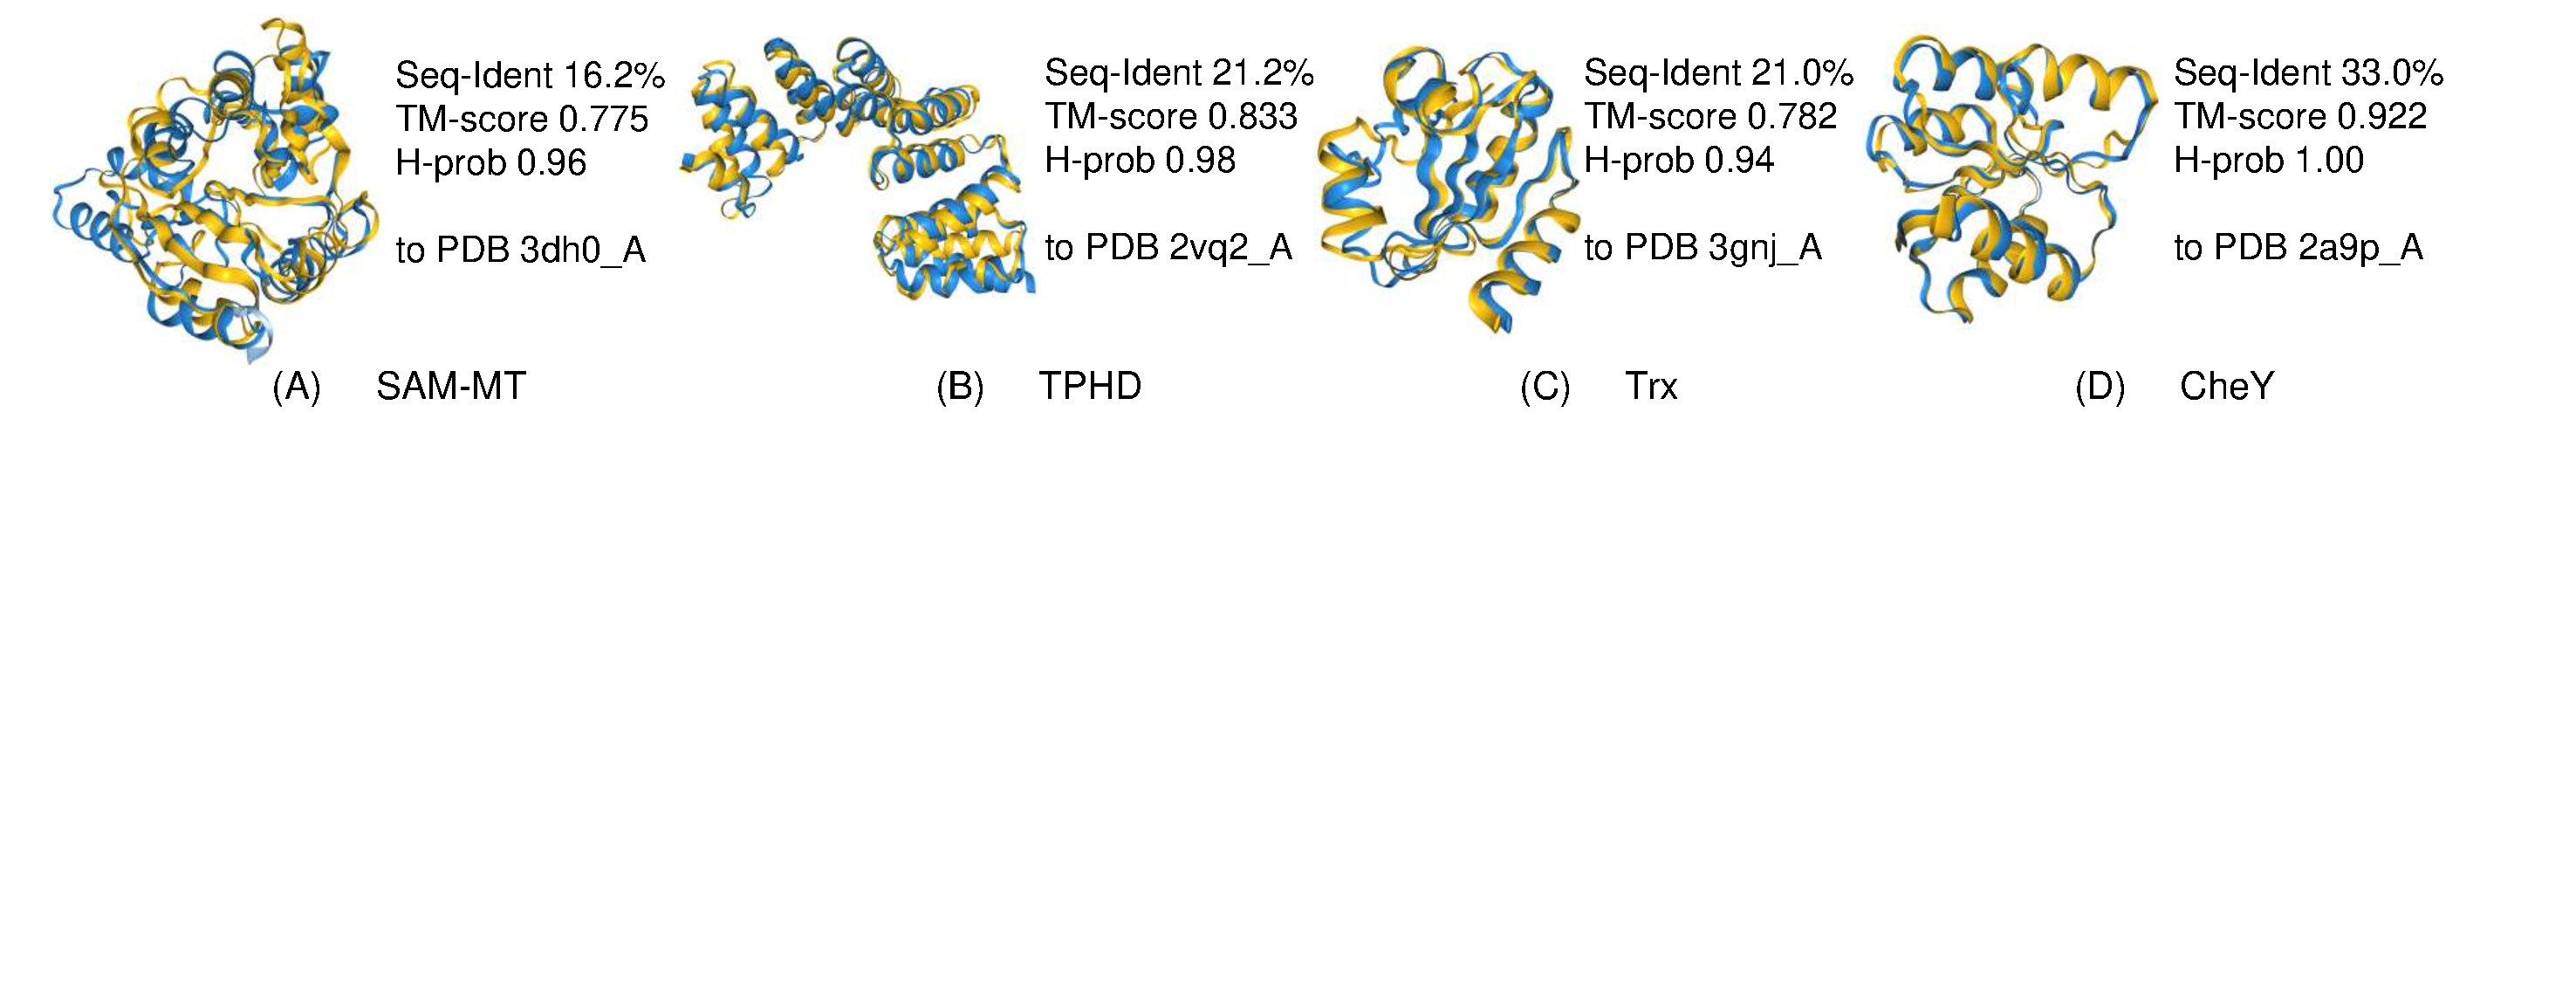
\includegraphics[trim={0 0 90em 0},clip,scale=0.4]{images/protein_visualization.pdf}
		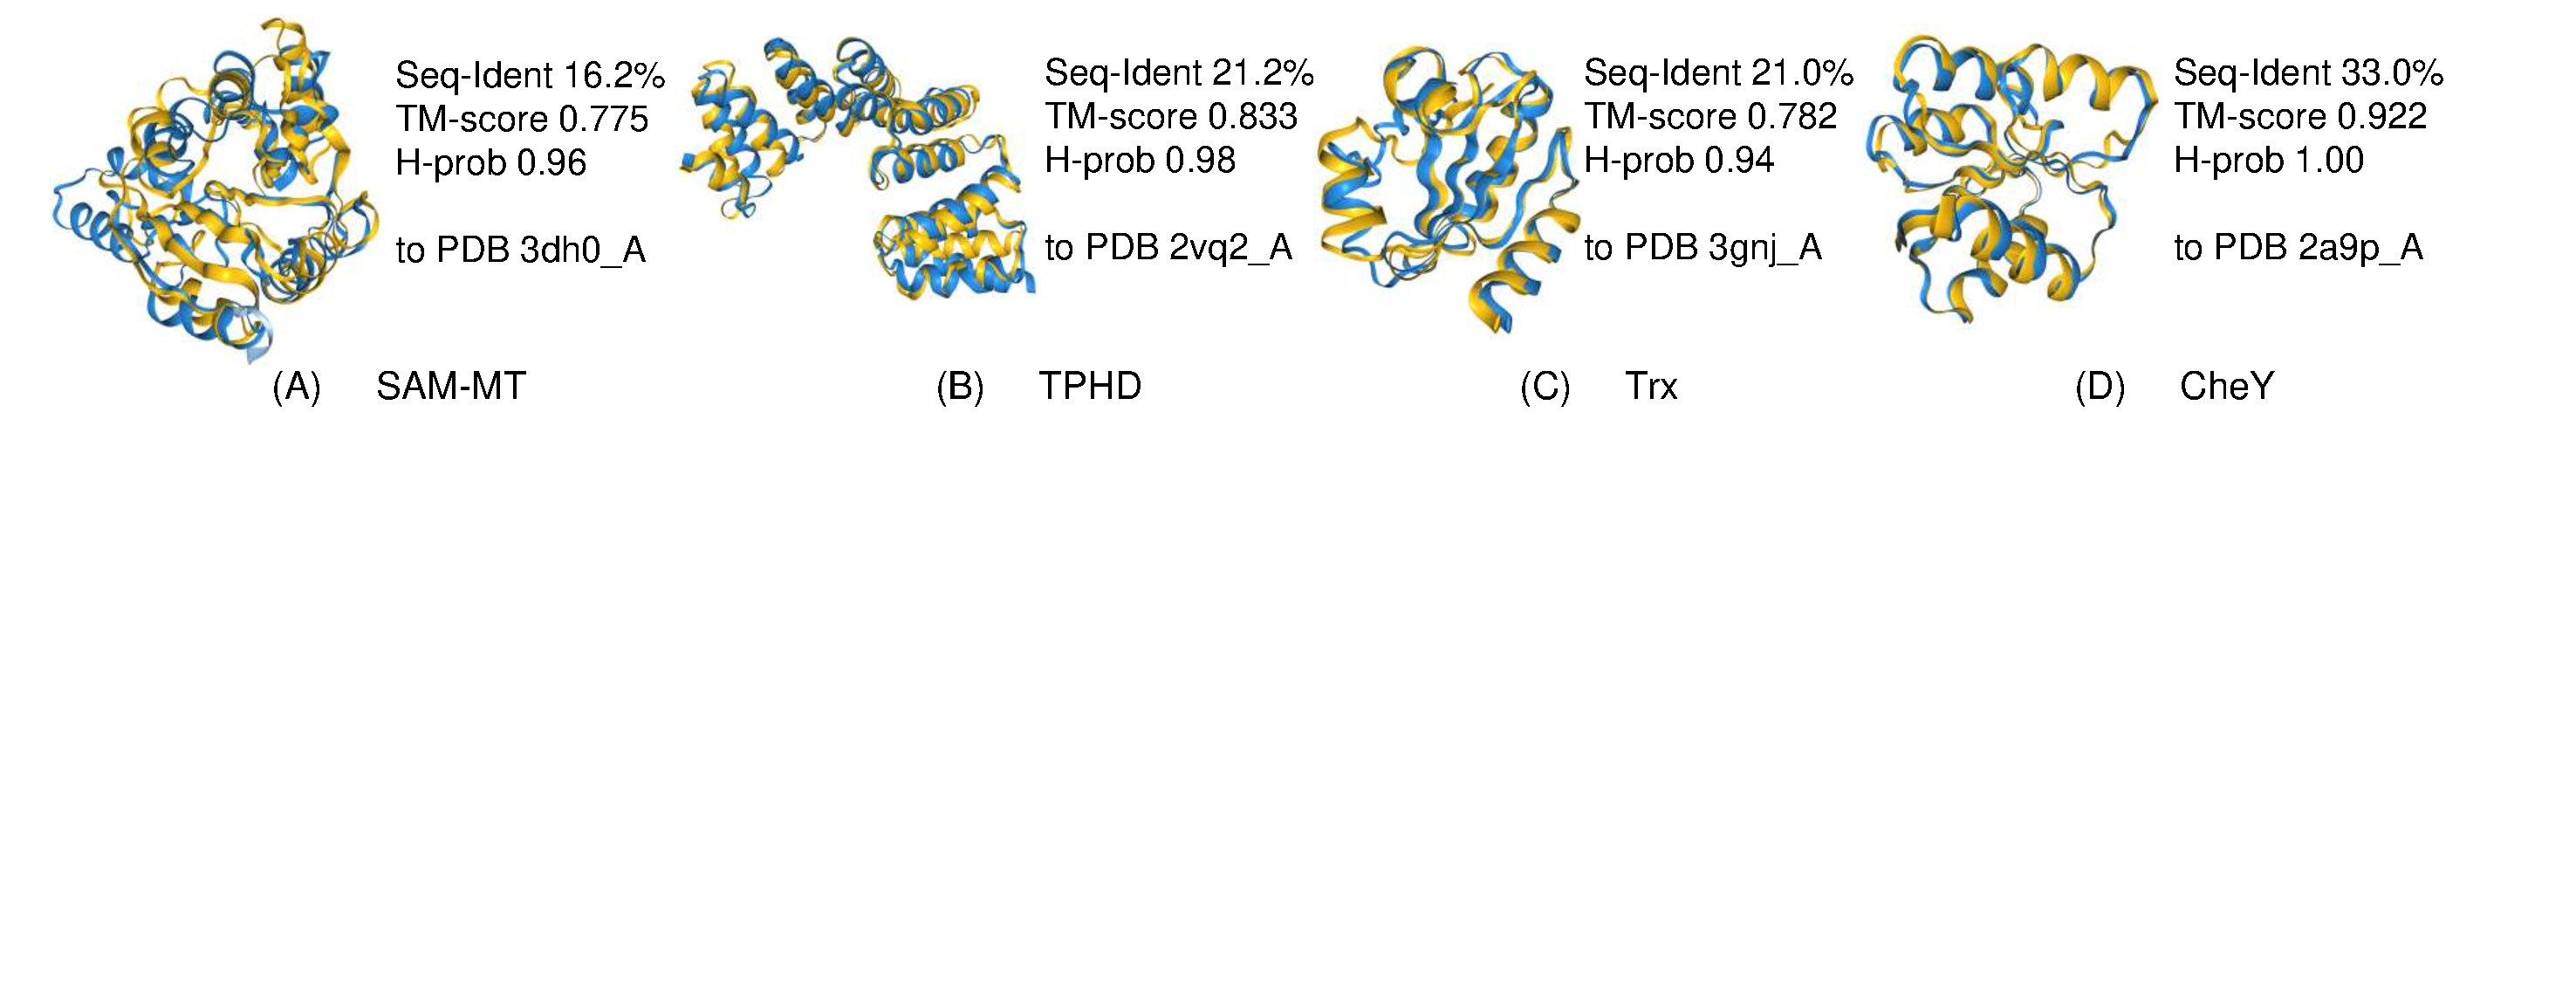
\includegraphics[trim={31.5em 0 57.4em 0},clip,scale=0.4]{images/protein_visualization.pdf}
		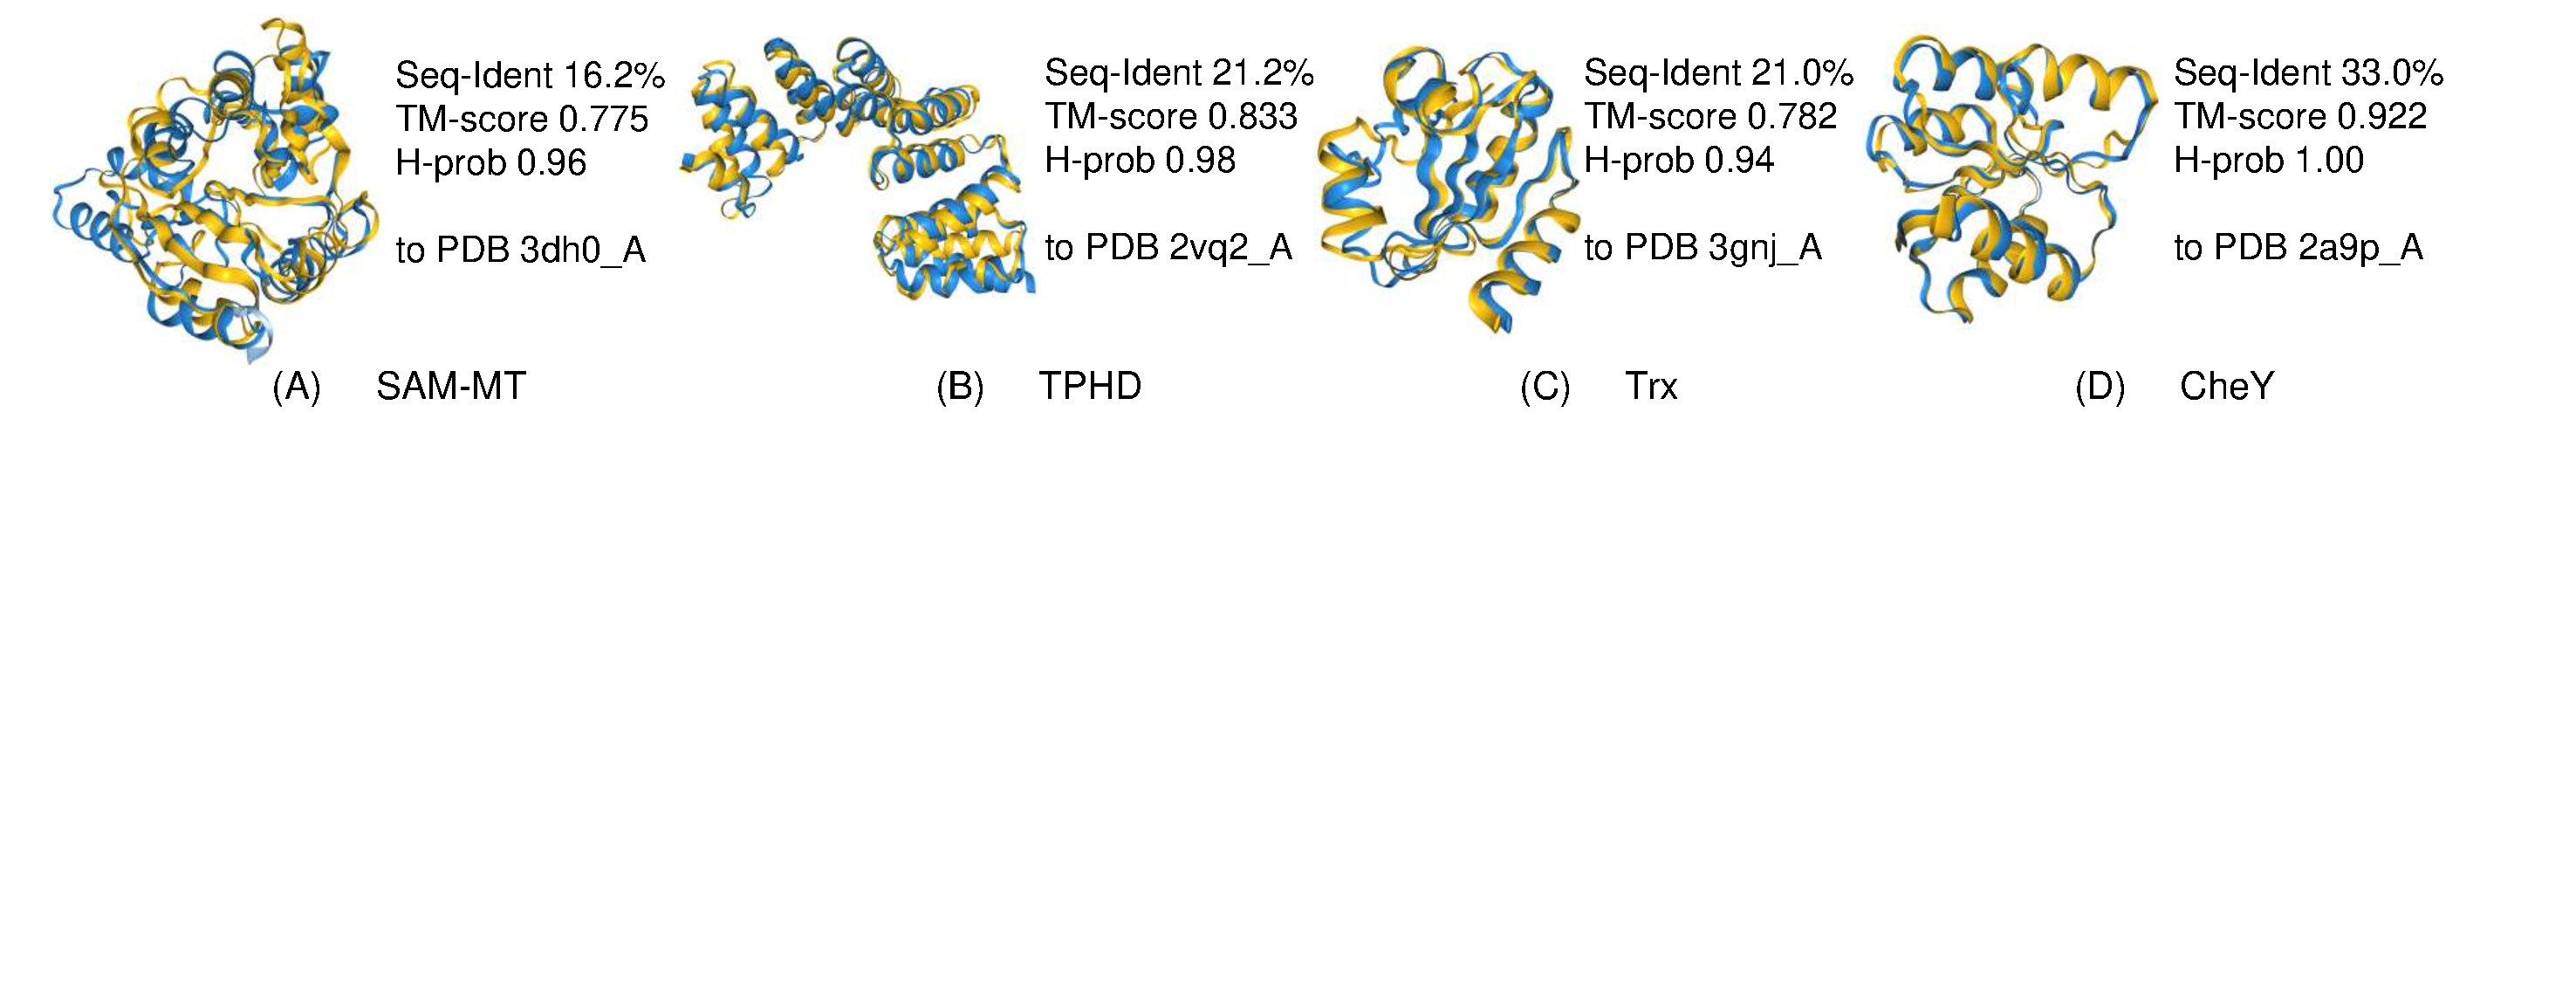
\includegraphics[trim={64em 0 30em 0},clip,scale=0.4]{images/protein_visualization.pdf}
		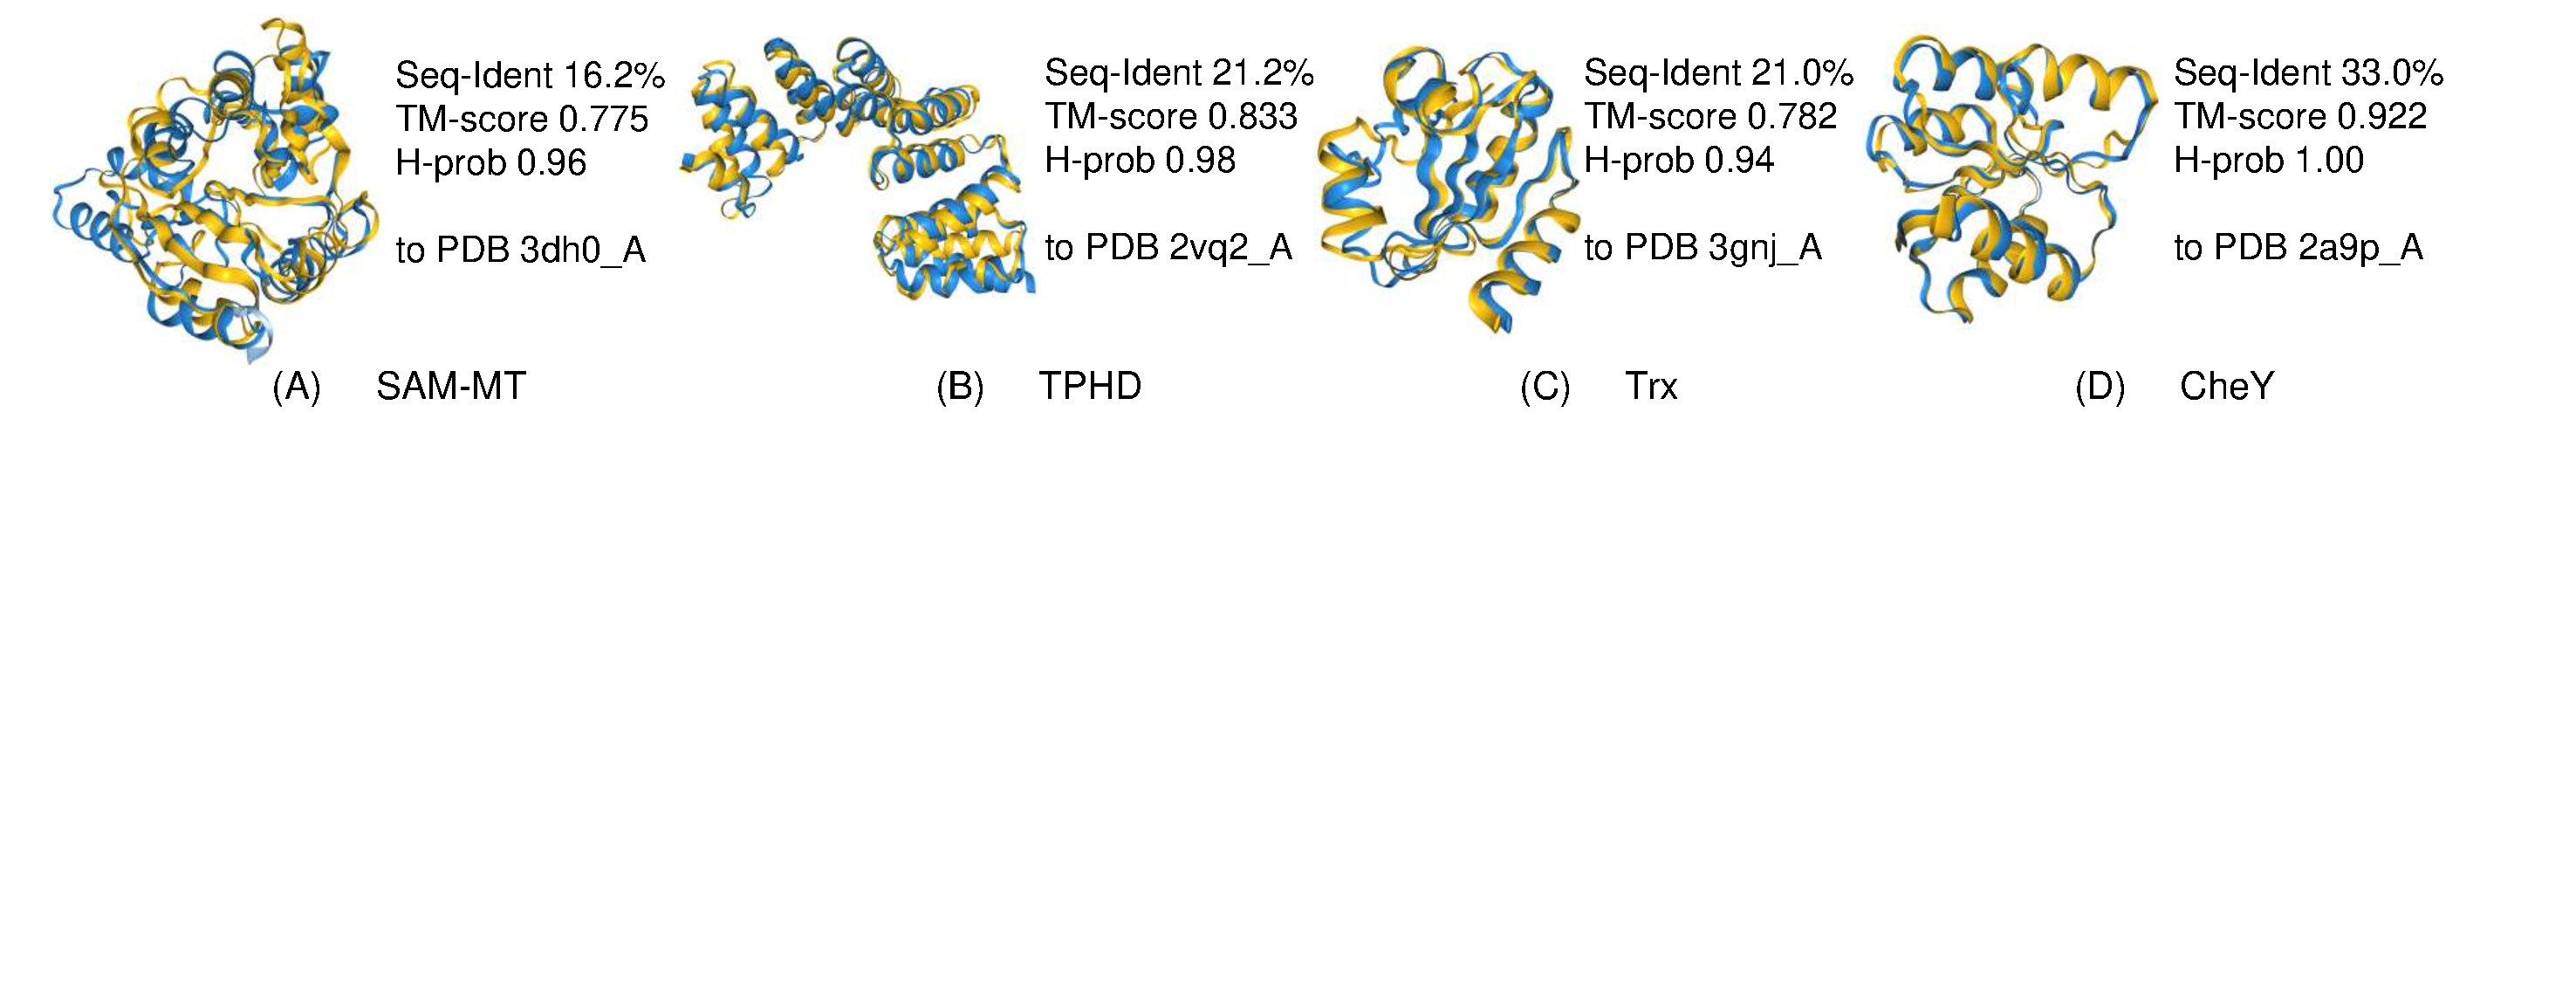
\includegraphics[trim={92em 0 0 0},clip,scale=0.4]{images/protein_visualization.pdf}
	\end{center}
\end{frame}

\begin{frame}{Natural Language Ability}
	\begin{center}
		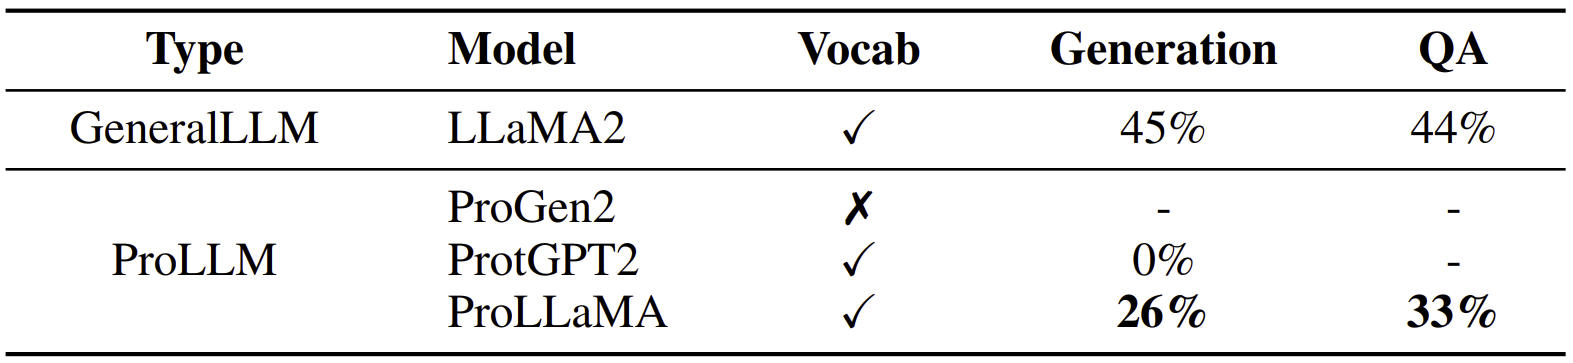
\includegraphics[scale=0.21]{tables/natural_language_ability_comparison.png}
	\end{center}
\end{frame}

\begin{frame}{Sequences Generated w/o Instructions - Distributions}
	\begin{center}
		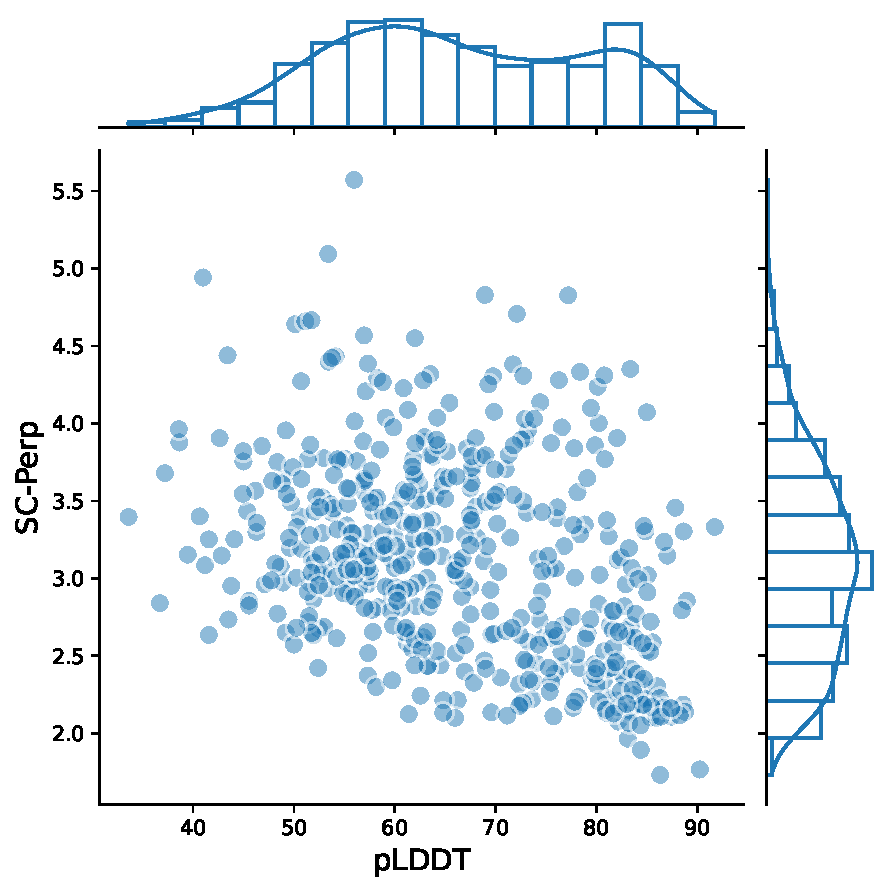
\includegraphics[scale=0.35]{images/plddt_scperp.pdf}
		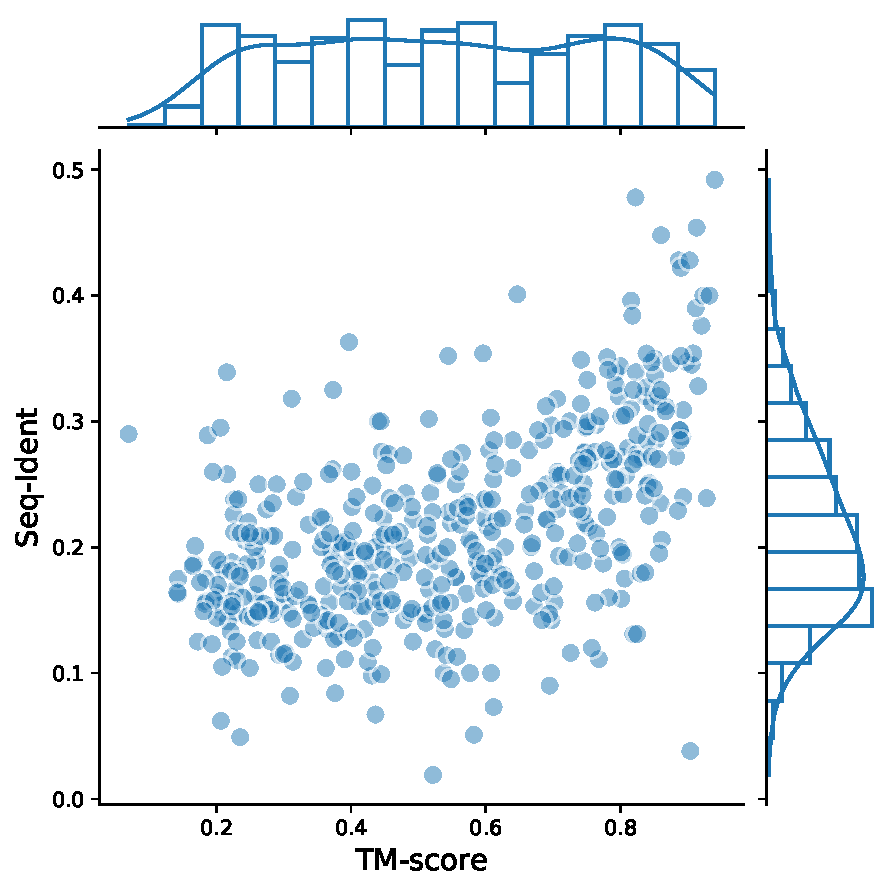
\includegraphics[scale=0.35]{images/tm_sid.pdf}
	\end{center}
	\begin{itemize}
		\item 1 spot = 1 sequence
	\end{itemize}
\end{frame}

%\begin{frame}{Outline}
%\tableofcontents
%\end{frame}

%\section{References}
%\begin{frame}[allowframebreaks]
%\frametitle{References}
%\printbibliography
%\end{frame}

\end{document}